% -*- mode: LaTeX; coding: utf-8 -*-
\documentclass[12pt]{article}
\usepackage[unicode,colorlinks]{hyperref}
\usepackage[T2A]{fontenc}
\usepackage[utf8]{inputenc}
\usepackage[russian]{babel}
\usepackage{amsmath}
\usepackage{amssymb}
\usepackage{eufrak}
\usepackage{epsfig}
%\usepackage[mathscr]{eucal}
\usepackage{psfrag}
\usepackage{tabularx}
\usepackage{wrapfig}
%\usepackage{eucal}
\usepackage{euscript}

\usepackage[usenames]{color}
\usepackage{colortbl} 

\definecolor{codegreen}{rgb}{0,0.6,0}
\definecolor{codegray}{rgb}{0.5,0.5,0.5}
\definecolor{codeblack}{rgb}{0.1,0.,0.3}
\definecolor{codeemph}{rgb}{0.5,0.1,0.5}
\definecolor{codepurple}{rgb}{0.58,0,0.82}
\definecolor{backcolour}{rgb}{0.95,0.95,0.92}

\usepackage{listings}\lstset{
	basicstyle=\ttfamily\fontsize{10pt}{10pt}\selectfont\color{codeblack},
  commentstyle=\color{codegray},
	keywordstyle=\tt\bf\color{codeemph},
	belowskip=0pt
    }

\setlength{\topmargin}{-0.5in}
\setlength{\oddsidemargin}{-5.mm}
\setlength{\evensidemargin}{-5.mm}
\setlength{\textwidth}{7.in}
\setlength{\textheight}{9.in}

\def\dfdx#1#2{\frac{\partial #1}{\partial #2}}
\def\hm#1{#1\nobreak\discretionary{}{\hbox{\m@th$#1$}}{}}
\newcommand{\Frac}[2]{\displaystyle\frac{#1}{#2}}

\def\sr#1{{\left<#1\right>}}
\def\m{\mathbf m{}}
\def\gplt{{\tt gplt}}
\def\gnuplot{{\tt gnuplot}}
\def\python{{\tt python3}}
\def\RACS{{\tt RACS}}
\def\png{{\tt .png}}
\def\pdf{{\tt .pdf}}

\begin{document}
\begin{center}
 { \Large\bf
Утилита gplt3 --- построение графиков\\ типографского качества из командной строки\\ с минимальными усилиями\\[5mm]
}

\large
\copyright Антон Иванов (2023)\\[2mm]

\normalsize
Институт прикладной математики им. М.В. Келдыша РАН\\[2mm]

\small рисунки с пингвинами \copyright Людмила Степкина 
\end{center}

\vfill

\tableofcontents

\newpage
\section{Введение}
\begin{wrapfigure}[5]{t}{.3\textwidth}
  \vphantom{.}
  \vspace{-1.5cm}

  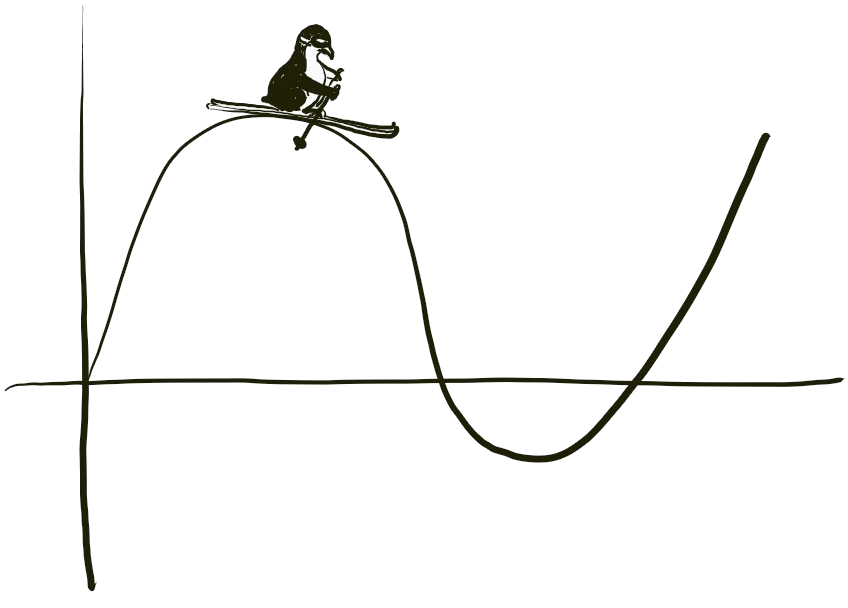
\epsfig{file=picts/gplt3/sin1, width=.27\textwidth}
\end{wrapfigure}

Первая версия утилиты \gplt{} появилась в начале нулевых годов, когда \gnuplot{} стал казаться автору слишком многословным.
На тот момент она называлась \verb'gnuplt' и была написана на \verb'bash'\footnote{Краткое описание той реликтовой версии утилиты можно найти в \cite{aiv:racs2007}.}.
С тех пор \gplt{} переписывалась несколько раз с нуля (при этом название скрипта становилось все короче),
сохраняя по возможности обратную совместимость с т.з. интерфейса.  

\def\gplt{{\tt gplt3}}

В настоящий момент утилита \gplt{} является скриптом на языке \python, разбирающим аргументы командной строки и формирующим команды для \gnuplot.
За счет коротких опций и различных умолчаний удается радикально уменьшить число нажатий клавиш. Кроме того, \gplt{}, как пылесос, собирает всю доступную информацию
(комментарии из заголовков файлов с данными и файлов .\RACS, \cite{aiwlib:SR:PP2018})
и старается на ее основе автоматически формировать метки к осям, подписи кривым и т.д.
Эта же информация позволяет давать столбцам имена и формировать из этих имен сложные математические выражения для построения.

Под графиками типографского качества понимаются графики с правильной шрифтовкой и зарамочным офррмлением (как минимум подписями к осям и кривым)~---
т.е. графики, которые могут быть  вставлены в печатную
работу не вызывая замечаний со стороны самого требовательного корректора. Несмотря на бурное развитие вычислительной техники, подготовка таких графиков по прежнему
остается коропотливой работой~--- утилита \gplt{} отчасти решает эту проблему.
Часть изменений в последней версии \gplt{} 2023 года как раз направлены на то, что бы упростить эту работу
еще больше за счет переиспользования введенных ранее команд. {\it<<Никакая информация не должна вводится в компьютер дважды!>>}~--- в \gplt эта идея возведена в абсолют.
При этом за один запуск \gplt{} способна сгенерировать целую серию рисунков с частично пересекающимися настройками.

Кроме рисования графиков на экране, \gplt{} может генерировать картинки в форматах \png{} и \pdf.  При генерации \pdf{}  файлов используется терминал {\tt esplatex}
из \gnuplot, затем результаты автоматически прогоняются через \LaTeX и у полученного файла обрезаются поля. С одной стороны, такой подход  обеспечивает правильную
шрифтовку и позволяет использовать выражения \LaTeX в подписях к осям и метках кривых. С другой стороны, вставка одного \pdf{} файла вызывает
значительно меньше проблем, чем вставка пары файлов \verb'.tex' и \verb'.eps' генерируемых терминалом {\tt esplatex} в \gnuplot.

Для каждого сгенерированного рисунка \gplt{} создает одноименный  файл с расширением \verb'.gplt3', содержащий набор опций для генерации рисунка.
Файл является запускаемым и при запуске создает рисунок заново, что может быть полезно если входные данные изменились.
Кроме того файл может скопирован под другим именем, отредактирован вручную и применен для создания другого рисунка\footnote{Будьте внимательны ---
  имя рисунка явно прописано в {\tt .gplt3} файле, не забывайте его изменять при редактировании!}.

Опыт автора показывает, что самой лучшей оболочкой для обработки результатов численного моделирования (особенно если речь идет об HPC) является командная строка
с правильным набором утилит~--- например \verb'yupiter' (\python3 с \verb'matlotlib') или \verb'matlab' оказываются в целом менее удобны, несмотря на свою <<заточенность>>
именно под такие задачи. Утилита   \gplt{} как раз является тем инструментом, который значительно расширяет возможности обычной комндной строки,
позволяя быстро просматривать полученные результаты (в т.ч.
без выкачивания их с удаленной машины, см. описание терминала \verb'sixel' в разделе ...) и сразу оформлять их в виде рисунков типографского качества. 

Утилита \gplt{} распространяется под лицензией Апач 2.0, т.е. относится к ПО с открытым программным кодом, но может использоваться в коммерческих проектах
без согласования с автором.

\section{Установка  и настройка утилиты}
\begin{wrapfigure}{t}{.3\textwidth}
  \vphantom{.}
  \vspace{-3cm}

  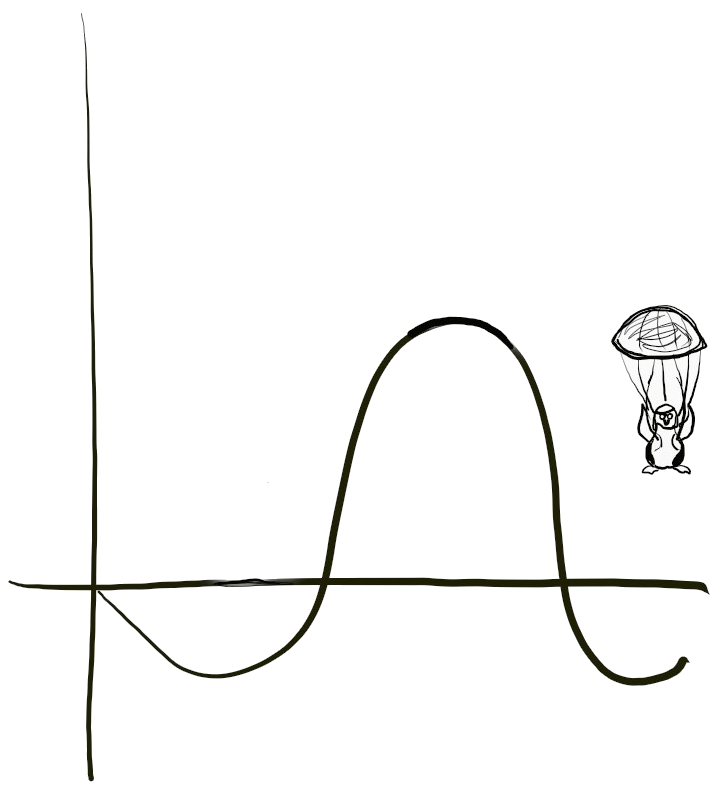
\epsfig{file=picts/gplt3/setup, width=.27\textwidth}
\end{wrapfigure}
Утилита \gplt{} написана для \verb'OS Linux', портирование под \verb'MS Windows' пока не проводилось. Скорее всего утилита будет работать
под \verb'MS Windows' в среде \verb'WSL', но автор не имеет возможности полноценно проверить эту гипотезу.

Хотя утилита \gplt{} является частью библиотеки \verb'aiwlib' \cite{aiwlib:SR:PP2018,aiwlib:SV2018,aiwlib:git},
тем не менее последняя версия выполнена в виде одного файла на языке \python, включающего в т.ч. достаточно подробную справку по утилите.
Такой подход несколько усложняет разработку (размер файла уже превысил 500 строк достаточно насыщенного кода), но значительно упрощает установку
неквалифицированными пользователями. Просто скопируйте \gplt{} в любую директорию из тропы поиска путей \verb'$PATH', например в \verb'~/bin':
\begin{verbatim}
$ mkdir ~/bin
$ export PATH=$PATH:~/bin
$ echo export PATH=\$PATH:~/bin >> ~/.bashrc
$ cd ~/bin && wget https://github.com/aivn/aiwlib/blob/master/bin/gplt3 
\end{verbatim}
Если у Вас уже есть директория \verb'~/bin/' и она присутствует в тропе поиска путей, можно ограничится последней строчкой.

При установке библиотеки \verb'aiwlib' утилита \gplt{} будет установлена автоматически.

Для нормальной работы утилита \gplt{} требует как минимум установленного \gnuplot. Для генерации \pdf{} файлов требуются \verb'pdflatex', \verb'epstopdf'
и \verb'pdfcrop'. 

Все настройки \gplt{} хранятся в необязательном конфигурационном файле  \verb'~/.\gplt3',
фалй может быть создан командой
\begin{verbatim}
$ gplt3 -dump-config-file
\end{verbatim}
и отредактирован.\\

\hrule
\begin{center}
\bf БУДЬТЕ ВНИМАТЕЛЬНЫ --- СТАРЫЙ ФАЙЛ С НАСТРОЙКАМИ,\\
ЕСЛИ ОН СУЩЕСТВУЕТ, БУДЕТ УНИЧТОЖЕН!
  \end{center}
\hrule
\phantom{.}

Файл содержит команды для запуска просмотрщиков \png{} и \pdf{} файлов, палитры для режима \verb'pm3d' и преамбулу \LaTeX{} документа для генерации \pdf{} файлов.

Кроме того, рекомендуется создать файл \verb'~/.gnuplot' cледующего содержания:
\begin{verbatim}
set colors classic
set style data lines
set ticslevel 0
set grid front
\end{verbatim}

\section{Вызов справки}
Для вызова справки запустите \gplt{} без аргументов или с аргументом \verb'-h'. По  опциям отмеченным символом \verb'(*)'
есть более подробная справка, для ее получения запустите
\begin{wrapfigure}[3]{t}{.3\textwidth}
  
\epsfig{file=picts/gplt3/help, width=.27\textwidth}
\end{wrapfigure}
\begin{verbatim}
$ gplt3 -h <опция>
\end{verbatim}
например
\begin{verbatim}
$ gplt3 -h -fn
\end{verbatim}

Утилита \gplt{} повзоляет выводить справку \gnuplot, для этого укажите интересующие пункты после опции \verb'-h',
подпункты указываются через точку, например
\begin{verbatim}
$ gplt3 -h expression.functions
----------------------------  expression.functions  ----------------------------
 Arguments to math functions in `gnuplot` can be integer, real, or complex
 unless otherwise noted.  Functions that accept or return angles (e.g. sin(x))
...
\end{verbatim}
Если Вы используете \gnuplot, возможно \gplt{} имеет смысл установить только для быстрого доступа к справке \gnuplot{} из командной строки.

Справка по многим опциям \gplt{} выводит справку по соответствующим опциям \gnuplot, например
\begin{verbatim}
$ gplt3 -h -sk
------------------------------------  -sk  -------------------------------------
 The `set key` command enables a key (or legend) containing a title and a
 sample (line, point, box) for each plot in the graph. The key may be turned off
...
\end{verbatim}

Интересующие опции и пункты справки \gnuplot{} (в т.ч. с подпунктами) могут указываться после опции \verb'-h' через пробел в любом порядке и количестве
(если листать вверх длинный вывод утомительно используйте перенаправление \verb'| less'), важно только что бы опция \verb'-h' шла первой.

В этом руководстве не очень много примеров~--- Вы всегда можете проверить интересующую Вас комбинацию опций самостоятельно, это быстро и безопасно. 

\section{Общие замечания}
\begin{wrapfigure}[5]{t}{.3\textwidth}
  \vphantom{.}
  \vspace{-3cm}

  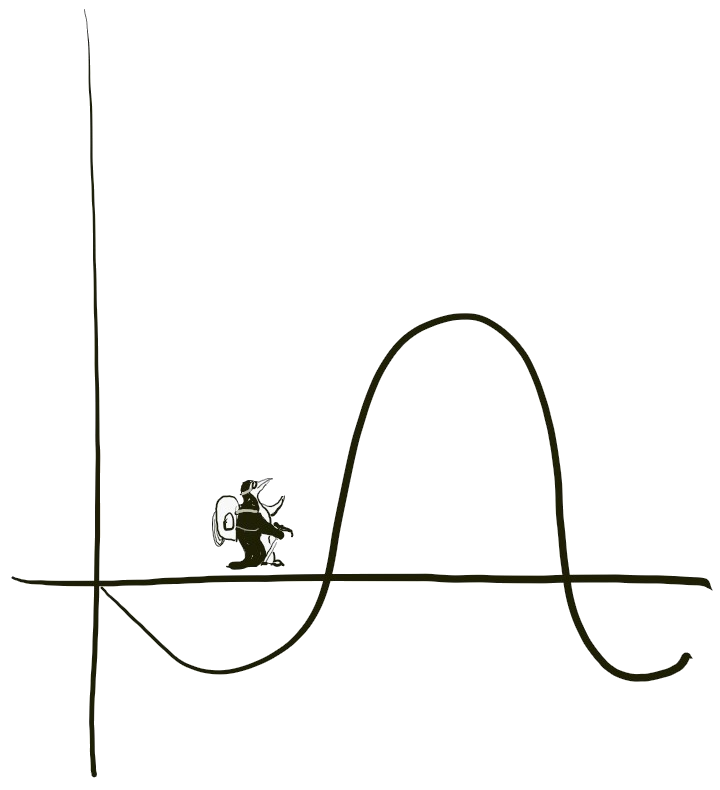
\epsfig{file=picts/gplt3/sin2, width=.27\textwidth}
\end{wrapfigure}
Утилита \gplt{} разбирает опции командной строки и формирует на их основе последовательность команд для \gnuplot. Если Вы хотите посмотреть
какая именно последоваельность команд будет отправлена в \gnuplot, добавьте опцию \verb'-debug' в (почти!) любое место~--- вместо \gnuplot{}
сформированная последовательность команд будет направлена на стандартный вывод:\footnote{Часть работы
  (чтение стандартного ввода, чтение заголовков файлов и т.д.) при этом будет все равно скрыта.}
\begin{verbatim}
$ gplt3 -fn x**2 -debug
set xlabel 'x'
set ylabel 'x**2'
plot x**2 notitle   
pause -1
\end{verbatim}

Синтаксис аргументов командной строки \gplt{} тривиален и может быть сформулирован в трех пунктах:
\begin{enumerate}
\item опции командной строки начинаются с одинарного знака <<минус>>;
\item некоторые опции командной строки имеют один (и только один) аргумент, если аргумент пуст то все равно надо указывать пустые кавычки \verb|''| или \verb|""|;
\item все, что не является опцией и аргументом опции, трактуется как имя файла с данными для отрисовки.
\end{enumerate}
\begin{verbatim}
$ gplt3 -nk          ...         -fn 'sin(x)'     ...     result.dat
        ^ опция без аргументов   ^ опция и ее аргумент    ^ файл с данными
\end{verbatim}
Порядок следования опций и файлов с данными не фиксирован, но {\bf может} иметь значение.  Некоторые опции имеют синонимы, например \verb'-U' и \verb'-u'
(задает кривые из файла для отрисовки) или \verb'-w' и \verb'-ds' (глобально задает стиль отрисовки).

По семантике все опции можно разделить на следующие группы.
\begin{enumerate}
\item Простые опции включающие/выключающие какой то режим (например \verb'-3d', \verb'-2d')
  и/или добавляющие команду для \gnuplot{} (например \verb'-sk <keyopt>' настраивает легенду передавая в \gnuplot{} команду \verb'set key <keyopt>').
  Самыми яркими представителями являются \verb'-s <command>' (просто передает в \gnuplot{} строку \verb'set <command>'),
  \verb'-us <command>' (передает \verb'unset <command>'), и совсем брутальная \verb'-raw <command>' передающая \verb'<command>'~---
  эти опции введены для каких то экзотических случаев и вообще говоря не рекомендуются для использования. 
\item Опции (с аргументами) явно устанавливающие подписи к осям~--- \verb'-lbx', \verb'-lby', \verb'-lbz', \verb'-lbcb', \verb'-lbx2', \verb'-lby2'
  и титул рисунка \verb'-ttl'. Аргументы этих опций обрабатываются специальным образом с учетом метаинформации (из заголовков файлов с данными и \verb'.RACS') и
  могут быть преобразованы в \LaTeX{}.
\item Опции задающие что именно рисовать и откуда:
  \begin{enumerate}
  \item \verb'-fn <function>' --- добавляет аналитическую функцию;
  \item \verb|-U '<expr1> <expr2> ...'| --- необязательная опция, задающая какие именно зависимости надо рисовать из файлов с данными, действует на {\bf все} файлы
    следующие после себя пока не встретится другая опция \verb'-U';
  \item собственно файлы с данными. 
  \end{enumerate}
\item Специальные опции определяющие логику работу \gplt{} и структурирующие последовательность аругментов в командной строке:
  \begin{enumerate}
  \item \verb'-to <filename>' --- терминирующая опция, отрисовывает все, что было накоплено с предыдущей опции \verb'-to', имя файла может иметь расширение \png, \pdf{}
    или быть пустым (\verb|""|, отрисовка на экран). Если последняя опция \verb'-to' не указана то она все равно будет вызыввна с отрисовкой на экран.
  \item \verb'-o <origin>' --- <<лайт>>-версия опции \verb'-to' внутри режима \verb'multiplot' (несколько графиков на одном рисунке). Включает режим
    \verb'multiplot', опция \verb'-to' соответственно создает рисунок со всеми графиками и выключает режим \verb'multiplot'.
  \item\verb'-i <filename>' --- модифицирует последовательность аргументов командной строки вставляя на свое место опции из файла \verb'<filename>',
    повторная вставка того же файла блокируется для защиты от зацикливания.
  \end{enumerate}
\end{enumerate}
Кроме того в \gplt{} есть циклы и макросы (см. раздел \ref{macroloops}), но они совершенно не обязательны к использованию, имеют свой синтаксис и пока что
о них можно не думать.

\section{<<Собачьи>> @-атрибуты}
\begin{wrapfigure}[5]{t}{.3\textwidth}
  \vphantom{.}
  \vspace{-2cm}

  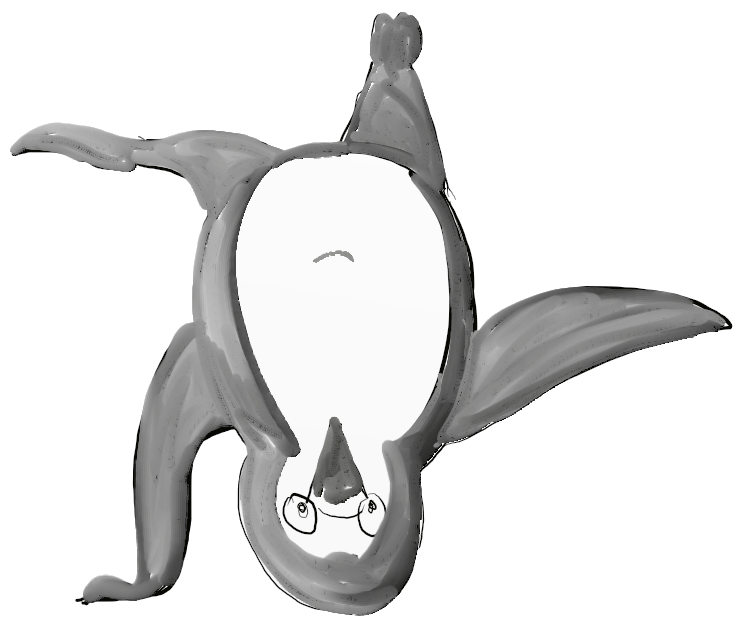
\epsfig{file=picts/gplt3/acrobat, width=.27\textwidth}
\end{wrapfigure}
В какой то момент во время эволюции и эксплуатации \verb'gplt' возникла острая необходимость для быстрого, точечного задания некоторых ключевых
параметров кривых~--- толщины, цвета и т.д. Как часто бывает, сделанный буквально <<на коленке>> вариант
оказался настолько удобным, что вытеснил другие, тщательно разрабатывавшиеся варианты. 

Что делать если мы договорились, что опция не может иметь больше одного аргумента, но именно этот аргумент мы иногда хотим дополнить каким то необязательными атрибутами,
причем сделать это как можно лаконичнее?
Разумеется расширить синтаксис. Для расширения синтаксиса в данном случае используется символ <<собака>> \verb'@', за которым через запятую дописываются те самые
дополнительные атрибуты. Например
\begin{verbatim}
$ gplt -fn x**2@5,blue,dots
\end{verbatim}
нарисует кривую $x^2$ голубыми точками размером в 5px.

Существует два типа @-атрибутов~--- для подписей к осям цвет, смещение и поворот; для кривых (аналитических функций,
имен файлов и аргументов опции \verb'-U') можно задавать толщину, цвет, стиль, оси отображения и подпись на легенде.
Все эти параметры так или иначе устанавливаются \gplt{} по умолчанию, @-опции нужны для явного и лаконичного исправления ситуации если что то пошло не совсем так. 

Важной особенностью @-атрибутов является их наследуемость, то есть если какой то из атрибутов не задан то он считается задаваемым по умолчанию
обычными алгоритмами \gplt, но ситуация может быть уточнена/исправлена в дальнейшем.
Как уже отмечалось выше, опция \verb'-U' задает одну или несколько кривых для отрисовки из следующих за ней файлов. При выводе на экран по умолчанию
все кривые рисуются линиями толщиной 1px, при выводе в файл 3px (на бумаге и/или в презентации линии кажутся тоньше).
Если указать \verb'-U x**2@5' то из последующих файлов будут строится кривые $x^2$ толщиной 5px, но если какой то из файлов задать как
\verb'filename.dat@2', то из него кривая $x^2$ будет построена с толщиной 2px~--- поскольку толщина линии для файла \verb'filename.dat' задается позже чем в \verb'-U',
то она имеет более высокий приоритет для данного файла, но не действует на остальные файлы. 

<<Собачьи>> @-атрибуты указываются после символа @ через запятую в произвольном порядке (едиственным исключенем является задание подписи к кривой на легенде,
она всегда указывается последней и начинается о знака \verb'='). 

Для подписей к осям доступны следующие @-атрибуты:
\begin{itemize}
\item смещение подписи/титула --- число;
\item цвет подписи/титула --- имя цвета;
\item поворот --- \verb'r<целое-число>'.
\end{itemize}
Например \verb'-lbx runtime@1.5,4,r90,red' установит по оси $x$ подпись \verb'runtime' красного цвета повернутую на $90^\circ$ со смещением в 1.5, 4.
Как уже отмечалось выше порядок следования атрибутов произвольный, \verb'-lbx runtime@1.5,red,r90,4' даст точно такой же эффект (но 1.5 должно идти раньше 4),
указывать можно не все атрибуты а только необходимые. 
Компоненты смещения задаются в единицах характерного размера символа, можно указывать не все компоненты а первые сколько-то необходимых (скажем только по $x$).
Важной особенностью является возможность указания только @-атрибутов без текста подписи, например \verb'-lbx @1.5,red,r90,4' задаcт смещение, цвет и поворот
подписи, но текст подписи будет определятся автоматически на основе выражений для отрисовки.

Ну и наконец \verb'-lbx ""' убирает подпись по оси $x$, \verb'-lbx <text>' устаналивает текст метки с атрибутами по умолчанию, 
\verb'-lbx @' возвращает полностью автоматический режим выбора текста подписи с атрибутами по умолчанию\footnote{Смещения нет, поворота нет, цвет черный.}.

Для выражений в \verb'-fn', \verb'-U' и для имен файлов доступны следующие @-атрибуты:
\begin{itemize}
\item толщина линии --- целое положительное число (по умолчанию 1 для выводва на экарн и 3 для отрисовки в файл);
\item цвет линии --- имя цвета (по умолчанию выбирается \gnuplot-ом, зависит от номера кривой на графике);
\item оси отображения --- \verb'x1y1', \verb'x1y2', \verb'x2y1', \verb'x2y2' (по умолчанию \verb'x1y1');
\item подпись к ривой на легенде --- начинается с \verb'=', должен идти последним (по умолчанию задается \gplt3{} на основе информации о том что именно рисуется);
\item стиль отрисовки --- все что не относится к предыдущим пунктам, вариантов \gnuplot{} предоставляет довольно много, например \verb'l' (\verb'lines'),
  \verb'p' (\verb'points') и т.д., см.
\begin{verbatim}
$ gplt3 -h style
...
Subtopics available for style:
    arrows            boxerrorbars      boxes             boxplot
    boxxyerror        candlesticks      circles           dots
    ellipses          errorbars         errorlines        filledcurves
    fillsteps         financebars       fsteps            histeps
    histograms        image             impulses          isosurface
    labels            lines             linespoints       lp
    points            polygons          rgbalpha          rgbimage
    steps             vectors           xerrorbars        xerrorlines
    xyerrorbars       xyerrorlines      yerrorbars        yerrorlines
    zerrorfill
\end{verbatim}
\end{itemize}

\section{Заголовки файлов с данными и другие источники метаинформации}
\begin{wrapfigure}[5]{t}{.3\textwidth}
  \vphantom{.}
  \vspace{-1.2cm}

  
\epsfig{file=picts/gplt3/table, width=.27\textwidth}
\end{wrapfigure}
Мы уже несколько раз упоминали заголовки \verb'.dat'-файлов, пора остановится на них поподробнее.

С точки зрения \gnuplot, все строчки в \verb'.dat'-файле начинающиеся с символа \verb'#', являются комментариями. С точки зрения \gplt{}
имеют значение строки начинающиеся с \verb'#:'
\begin{verbatim}
# пример заголовка для gplt3
#: R = 8.31   # универсальная газовая постоянная
#: rho_H2O, C_H2O = 1e3, 4200  # плотность и теплоемкость воды
#: rho_Fe = 7800;  C_Fe = 460  # плотность и теплоемкость железа
#: t rho T mu
#: mu.tex = '\\omega_1'  # задаем LaTeX представление для mu
0. 12  1e-3  14
...
\end{verbatim}
Здесь представлено задание пяти параметров ($R$, $\rho_{\rm H2O}$, $C_{\rm H2O}$, $\rho_{\rm Fe}$, $C_{\rm Fe}$) и задание имен для четырех столбцов файла с данными.
Чтение заголовка прекращается после первой же строки с данными (числами), дальше \gplt{} заглядывать не будет. В задаваемых через опцию \verb'-U'
выражениях к столбцам можно будет обращаться по именам, при конвертации в формат \gnuplot{} для отрисовки они будут выглядеть как \verb'($1)', \verb'($2)' и т.д.
Порядок следоваия при задании имен столбцов и параметров не имеет значения~--- можно указывать имена столбцов в начале, а параметры в конце, или задавать имена столбцов
где то между строчками с заданием параметров. Строки с заданием параметром (такими считаются строки начинающиеся с \verb'#:' и содержащие знак \verb'=')
обрабатываются функцией
\begin{verbatim}
exec(src_line, {'__builtins__': None}, dst_scope)
\end{verbatim}
и попадают в словарь \verb'dst_scope'. Глобальное пространство имен вида \verb|{'__builtins__': None}| обеспечивает безопасность отключая все
встроенные функции \python{}, т.е. код
\begin{verbatim}
#: import os; os.system('rm -rf ~/')
\end{verbatim}
не будет выполнен\footnote{<<Можно придумать защиту от дурака, но только от неизобретательного>> {\it Закон Нейсдра.}}. 


В последней строке заголовка задается \LaTeX{} версия для имени столбца \verb'mu', на экране и \png{} рисунках эта переменная
будет выглядеть как \verb'mu', на рисунках \pdf{} как $\omega_1$ (такое различие в обозначениях не кажется хорошей идеей, это просто пример).
Важно, что \verb|'\\omega_1'| это именно строка (в кавычках), и что там стоит именно два бэкслэша \verb'\\' (первый бэкслэш экранирует второй).
Аналогичный результат можно было бы получить написав \verb|r'\omega_1'|. Обрамление в \verb|r'$\omega_1$'| здесь не требуется и напротив будет являтся
ошибочным~--- \gplt{} расставляет \$ сам.
%Особенно важно то, что задание \verb'#: mu.tex = ...' идет {\bf после}
%задания имен столбцов~--- до этого момента имя \verb'mu' не определено не определено как имя столбца.
В старых версиях \verb'gplt' необходимо было указывать \LaTeX{} версии имен столбцов после того, как имена столбцов заданы.
В \gplt{} этот порядок уже не имеет значения, строки с заданием имен столбцов в любом случае обрабатываются в первую очередь.
Не спешите задавать \LaTeX{} версии имен столбцов~--- \gplt{} генерирует их самостоятельно в большинстве простых случаев.

Число имен в строке задающей имена столбцов не обязательно должно совпадать с числом столбоцов с данными~--- если имен будет меньше, Вы не сможете обратится к
последним столбцам (на самом деле сможете, но по другому), если имен будет больше, при обращении к несуществующему столбцу \gnuplot{} выдаст ошибку.
Допустимо задание нескольких вариантов имен столбцов в нескольких разных строках, это приведет к тому, что у столбцов будет по нескольку имен.
Если какое то имя будет продублировано, актуальным будет последняя версия имени:
\begin{verbatim}
#: A B C
#: C D E
\end{verbatim}
В этом странном примере к первому столбцу можно обращаться по именам \verb'A' и \verb'C', ко второму  \verb'B' и \verb'D', к третьему только \verb'E'.
При построении этого файла по умолчанию (без опции \verb'-U') акутальным с точки зрения подписей к осям будт последний комплект имен столбцов. 

По умолчанию, с точки зрения \gplt,  первые три столбца имеют имена \verb'x', \verb'y', \verb'z', кроме того первые 255 столбцов имеют имена \verb'C1' ... \verb'C255',
имя \verb'C0' обозначает номер строки и на сегодняшний день это единственный способ обратиться к номеру строки. 

В \gplt{} можно задавать столбцы как компоненты вектора, например
\begin{verbatim}
#: t E.x E.y E.z P 
\end{verbatim}
или
\begin{verbatim}
#: t E[0] E[1] E[2] P 
\end{verbatim}
или даже
\begin{verbatim}
#: t E[] E[] E[] P 
\end{verbatim}
Здесь \verb't' и \verb'P' --- обычные скалярные параметры, \verb'E' векторный параметр.
В первом случае имена у компонент вектора могут быть любыми индентификаторами, обращаться к компонентам в выражении можно
по именам (через точку), или по номерам, в том порядке в котором они были указаны, как \verb'E[0]' вместо \verb'E.x' и т.д.
Во втором и третьем случаях обращаться к компонентам в выражении можно только по номерам.
Во случае последовательность компонент
 вектора может быть любой, но важно, что бы номера компонет были от $0$ до $D-1$, где $D$~--- размерность вектора. В третьем случае
 номера компонентам вектора будут розданы автоматически, начиная с нуля.
Во всех случаях компоненты могут идти в перемешку с обычными скалярными параметрами
\begin{verbatim}
#: t E.x P E.y E.z  
\end{verbatim}
или
\begin{verbatim}
#: t E[0] P E[1] E[2]
\end{verbatim}
или даже
\begin{verbatim}
#: t E[] P E[] E[]  
\end{verbatim}
хотя это и будет выглядеть странно.
В выражениях, кроме обращения к компонентам вектора, можно брать модуль вектора как \verb'E.abs()' или \verb'abs(E)', скалярно перемножать вектора при помощи \verb'*',
умножать вектор на скаляр и скаляр на вектор при помощи \verb'*', складывать и вычитать вектора, а так же вычислять векторное произведение при помощи \verb'%'.

Неоднократно упоминавшиеся файлы \verb'.RACS' содержат словарь с параметрами расчета в формате \verb'pickle'. Эти файлы создаются \verb'RACS' (системой контроля результатов и алгоритмов,~\cite{aiwlib:SR:PP2018}). Каждый раз обрабатывая файл с данными \gplt{} ищет файл \verb'.RACS' вверх по дереву директорий начиная от директории содержащей файл с данными
и вплоть до корня файловой системы. Параметры из файла \verb'.RACS' могут быть использованы в различных выражениях, включая подписи к кривым на легенде и
заголовок рисунка. 

\section{Ввод и преобразование выражений, автоматическая генерация подписей}
\begin{wrapfigure}[8]{t}{.3\textwidth}
  \vphantom{.}
  \vspace{-1.7cm}

  
\epsfig{file=picts/gplt3/quest, width=.27\textwidth}
\end{wrapfigure}
Это наверное самый важный и сложный для понимания раздел руководства, но в тоже время самый интересный. 

Выражением здесь мы будем называть некоторое алгебраическое выражение, например $a x$, $2$, $A + B\sin^2\omega t$ и т.д. Выражение всегда вводится
в синтаксисе \python{} {\bf без} пробелов\footnote{При задании аналитической функции через {\tt -fn} и в подписях к осям/титуле пробелы не страшны если они
  заэкранированы от {\tt bash}, но для опции {\tt -U} пробелы являются разделителями аргумента!}, например \verb'a*x', \verb'2', \verb'A+B*sin(omega*t)**2' и т.д.

Сразу отметим, что \gplt{} несколько расширяет синтаксис \python{} вводя дополнительные скобки (в обычном, алгебарическом смысле) как
\verb'(%...%)', \verb'[%...%]', \verb'', \verb'<%...%>', \verb'' и \verb'|%...%|', где под \verb'...' понимается законченный фрагмент выражения.
Забранный в скобки фрагмент выражения как обычно может являтся частью большого выражения, но его скобки будут выводится всегда при отображении в текст, например
\verb'a*[%(%b%)+(c*d)%]' даст в \LaTeX\linebreak $a[(b)+cd]$~--- обратите внимание, что здесь \verb'(c*d)' выводится без скобок, поскольку они не требуются
с т.з. приоритета операций. При выводе в \LaTeX{} к скобкам добавляются \verb'\left' и \verb'\right'. Скобки \verb'|%...%|' трактуются как модуль,
в том числе и при конвертации выражения в \gnuplot{}, а функции \verb'abs(...)' и \verb'fabs(...)' воспринимаются как \verb'|%...%|'.

Доступны все операции \python{}, операция \verb'//' тракутется как обычное деление но при выводе в \LaTeX{} конвертируется во \verb'\frac'.
Операция \verb'^' воспринимается {\bf не} как степень а как побитовый \verb'xor'.

Пеобразование выражений действует по одному и тому же алгоритму (с небольшими нюансами)~--- после обработки расширенного синтаксиса скобок выражение преобразуется в AST
(абстрактное синтаксическое дерево), затем полученная структура может быть преобразована к одному из трех форматов~--- \gnuplot{} (для генерации
строки \verb'plot ...'), текстовому (для отображения на экране или в \png{} файл) или \LaTeX{} (для генерации \pdf).
AST состоит из экземляров классов реализующих операции \python, по одному классу на каждую операциию (\verb'AddOp' для \verb'+', \verb'MulOp' для \verb'*'
и т.д., \cite{aiv:symbalg:MM2015}),
классы определены непосредственно в теле утилиты \gplt. Разбор выражения \verb'expr' производится при помощи функции
\begin{verbatim}
eval(expr, {'__builtins__': None, ... globalscope...}, {...localscope...})
\end{verbatim}
из соображений безопасности все встроенные функции \python{} при этом отключены. В глобальном конктесте \verb'globalscope' размещаются математические функции:
\begin{verbatim}
  abs   fabs acos acosh airy  asin  asinh atan   atanh   ceil     cos    cosh ch   
  ctg   cth  erf  exp   floor gamma int   inverf invnorm lambertw lgamma log  ln
  log10 lg   norm sgn   sin   sinh  sh    sqrt   tan     tg       tanh   th 
\end{verbatim}
подробнее см. \verb'$ gplt3 -h expressions.functions plot'. Все самое интересное связано с локальным контекстом \verb'localscope'.


AST для выражения это ациклический направленный граф, листьями AST являются числа или переменные. 
Есть два разных режима преобразования выражений (зачастую одного и того же выражения):
\begin{itemize}
\item преобразование выражения в формат \gnuplot{} для фунцкии \verb'plot',  в этом случае все переменны должны быть заменены на числа или на номеров столбов
  в виде \verb'($1)', \verb'($2)' и т.д.;
\item преобразование выражения для подписи в форматы \verb'txt' или \LaTeX{}, в этом случае напротив, вместо чисел желательно испольщовать имена переменных,
 при выводе в \LaTeX{} нужно по возможности дать именам переменных их \LaTeX-версии, например заменить \verb'omega0' на \verb'\omega_0'.
\end{itemize}
Кроме формата вывода, эти режимы отличаются содержимым \verb'localscope', причем это отличие принципиальное~--- если в первом режиме
использование неизвестной переменной должно приводить к ошибке, то во втором режиме использование произвольного набора имен вполне допустимо.
В первом режиме \verb'localscope' это словарь, содержащий переменные ассоциированные с параметрами расчета полученными из файла~\verb'.RACS',
заголовка \verb'.dat'-файла и номерами столбцов \verb'.dat'-файла. Во втором режиме все переменные, даже те которые ассоциированы с параметрами расчета (числа)
отображаются под своими именами для наглядности. Кроме того, при выводе в \LaTeX{} для наглядности рациональные числа хорошо выводить в виде дробей,
если числитель и знаменатель по модулю не превышают девяти, например \verb'0.333333333333333' будет заменено на $\frac13$.

Можно сформулировать следующие правила относительно переменных при задании выражений для {\bf отрисовки}.
\begin{enumerate}
\item При задании обычной функции (опция \verb'-fn') аргументами функции могут являться переменные $x$ в \verb'-2d' случае или  $x, y$ в \verb'-3d' случае.
\item При задании параметрической функции (опция \verb'-fn' где то перед которой стоит опция \verb'-par')
  аргументами функции могут являться переменные $t$ в \verb'-2d' случае или  $u, v$ в \verb'-3d' случае. Во всех случаях параметрическая функция задается как
  кортеж выражений (выражения следуют через запятую), число элементов кортежа должно отвечать размерности графика:
\begin{verbatim}
$ gplt3 -par -fn 'sin(t),cos(t)'                            # окружность
$ gplt3 -par -3d -fn 'sin(u)*sin(v),cos(u)*sin(v),cos(v)'   # сфера
\end{verbatim}
\item При задании кривых для отрисовки из файла (опция \verb'-U', несколько кривых должно быть отделены пробелом и в этом случае обязательны кавычки поскольку с т.з.
  шелл это должен быть аргумент опции) в качетсве аргументов можно использовать любые имена столбцов, в том числе имена столбцов по умолчанию.
\begin{verbatim}
$ echo "#: a, b = 1, 2.5" > test1.dat 
$ echo "#: A B C" >> test1.dat 
$ python3 -c 'for i in range(100): print(i, i**2, i**3)' >> test1.dat
$ gplt3 test1.dat             # кривая B(A), кавычки не обязательны.
$ gplt3 -U 'a*B C' test1.dat  # кривые (2*B)(A) и C(A), здесь кавычки обязательны!
\end{verbatim}
\item По умолчанию при отрисовки из файла по осям $x$ (и $y$ в \verb'-3d' случае) откладываются знаяени из первого (и второго в \verb'-3d' случае) столбцов.
  Аргументы кривой можно именить указав новые аргументы в скобках, как для обычной функции, лучше взять выражение в скобки:
\begin{verbatim}
$ gplt3 -U 'С C(B) (A+2*C)(B**2)' test1.dat  # кривые C(A) и т.д.
\end{verbatim}
\item Можно задавать кривую в \verb'-U' как кортеж в порядке возрастания осей, т.е. вместо \verb|-U 'C(B)'| писать \verb'-U B,C'. При использовании
  стилей требующих много компонент (например \verb'errorbars') это единственный способ указать все необходимые компоненты. Кортеж транслируется в выражение
  для \gnuplot{} через \verb':' (попробуйте добавить опцию \verb'-debug').
\item Все остальные символы в выражениях должны быть параметрами из заголовков \verb'dat'-файла или \verb'.RACS'. 
При задании функции доступны все параметры из использованных ранее на этом графике \verb'dat'-файлов и связанных с ними \verb'.RACS'.
\begin{verbatim}
$ gplt3 -fn a+b*x  test.dat  # ошибка, a и b неопределены
$ gplt3 test.dat -fn a+b*x   # кривые B(A) и 1+2.5*x, фактически 1+2.5*A
$ gplt3 test.dat -to '' -fn a+b*x  # ошибка, после -to уже нет a и b
\end{verbatim}
Если есть несколько файлов с перекрывающимися параметрами, актуальными являются значения параметров из последнего файла
\begin{verbatim}
$ echo "#: b, c = -3, 4" > test2.dat 
...
$ gplt3 test1.dat test2.dat -fn a+b*x+c*x**2  # функция 1-3*x+4*x**2
\end{verbatim}
\end{enumerate}

При явном задании подписей  действуют другие правила.
Мы будем говорить о правила преобразования некоторого выражения \verb'epxr' встречающегося в аргументах опций
\verb'-lbx', \verb'-lby', ... (подписи к осям),  \verb'-ttl' (титул графика) и @-атрибутах \verb'-U' и \verb'-fn' после знака \verb'='
(явное задание подписей кривых на легенде).   
\begin{enumerate}
\item Как и в предыдущем случае, выражение должно быть введено в расширенном (за счет скобок) синтаксисе языка \python,
  затем оно будет преобразовано к AST при помощи \verb'eval'. Если такие преобразования не нужны, то в конце выражения
  нужно поставить \verb'!'~--- тогда оно останется без изменений при выводе на экран/в \png, при построении \pdf{} в выражении
  должно будут заэкранированы специальные символы \LaTeX{}\footnote{Идеальным было бы применение {\tt $\backslash$verb}, но через терминал {\tt epslatex}
    это не работает в сложных случаях}. Например 
  Если никакие преобразования не нужны, в конце выражения нужно поставить \verb'!!'. Если Вам нужен \verb'!' в конце выражения сам по себе,
  добавьте после него пробел~--- в любом случае в этом случае с т.з. шелл будут нужны кавычки.
\item При задании подписей функций и кривых из файлов действуют теже правила относительно параметров, что и при создании выражений для отрисовки~---
  кривая из файла <<видит>> все параметры из заголовка файла и связанных (лежащих в той же директории или выше) с ним файлов \verb'.RACS',
  функция имеет доступ к сводному словарю параметров кривых из всех предыдущих файлов. При задании подписей к осям и титула графика
  доступен сводный словарь с параметрами всех файлов графика.
\item Все параметры в выражении подставляются в виде чисел.  Все неизвестные имена параметров остаются как имена, по возможности для них генерируются \LaTeX{}-версии.
  Если имя заканчивается символом \verb'_' то этот символ отбрасывается, что позволяет реализовывать следующие конструкции:
\begin{verbatim}
$ gplt3 test{1,2}.dat@=b_==b  # две кривых B(A) с подписями 'b==2.5' и 'b==-3'
\end{verbatim}
\item   При выводе в \LaTeX{} все рациональные дроби в выражении
  с числителем и знаменателем меньше 10 по модулю приводятся к виду $\frac ab$, например \verb'0.3333333333333' будет заменено на $\frac13$.
\end{enumerate}

Если подпись к какой либо оси не задана явно, \gplt{} пытается сгенерировать ее автоматически.
При этом каждая кривая (кривая из файла или функция) рассматривается как кортеж выражений отображаемых по осям.
Для кривых из файлов тут все однозначно, для функций в не-параметрическом режиме для осей $x$ (и $y$ в \verb'-3d')
рассматриваются либо соотвествующие элементы выражения для последней кривой из файла (если есть), либо 
переменные $x$ и $y$. Старайтесь размещать фукции после кривых из файлов, это дает \gplt{} больше информации.
Затем, для каждой из осей группируются соотвествующие выражения. дубликаты выбрасываются, а оставшиеся выражения отображаются через запятую.

При автоматическом построении подписей к кривым на легенде действует один из четыре режимов;
\begin{enumerate}
\item если кривая одна --- легенда никогда не отображается, считается что подписей к осям достаточно;
\item если у всех кривых из файлов совпадают выражения --- отображаются только пути к файлам;
\item если на графике две кривых, одна из них из файла а другая функция --- легенда будет иметь вид \verb'calc' для файла и \verb'theor' для функции;
\item иначе отображается полная информация --- путки к файлам и выражения для кривых из файлов, выражения для функций.
\end{enumerate}
При отображении путей к файлам по возможности отбрасываются совпадающие начала и концы путей, если отбрасывается только часть имени (директории)
то отброшенная часть заменяется на ...
(многоточие).

\section{Циклы и макросы}\label{macroloops}
\begin{wrapfigure}[7]{t}{.3\textwidth}
  \vphantom{.}
  \vspace{-2.7cm}

  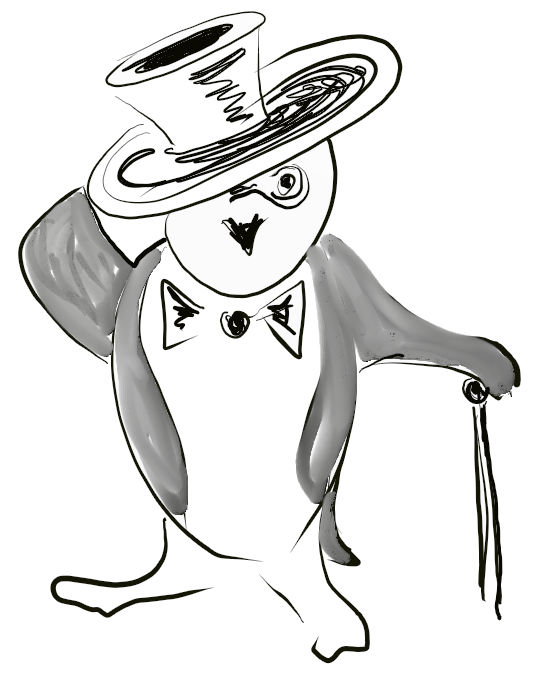
\epsfig{file=picts/gplt3/hat1, width=.27\textwidth}
\end{wrapfigure}
Циклы и макросы в \gplt{} предназначены для создания серий сложных рисунков за один запуск утилиты, показа анимации и т.д.
Есть целых два варинта задания макросов и один вариант для циклов.
Кроме показа анимации, основная мотивация дл ввежения циклов и макросов в \gplt{} все та же~--- {\it никакая информация не должна вводится в компьютер дважды}.
Необхожимоть дублировать ввод информации неизбежно увеличивает трудозатраты и приводит к ошибкам.

В \python.8 была введена новая операция \verb':=' <<морж>> (значок и правда похож на моржа).
В некоторых случаях эта операция значительно укорачивает код и делает его гораздо нагляднее.
В \gplt{} есть точно такой же \verb':=' <<морж>>. Эта операция применяется к аргументам любых опций
и позволяет использовать эти аргументы многократно.  Например необходимо ввести
\begin{verbatim}
$ gplt3 ... longfilename.dat ... longfilename.dat ... longfilename.dat ...
\end{verbatim}
Вместо этого можно ввести 
\begin{verbatim}
$ gplt3 ... lf:=longfilename.dat ... lf ... lf ...
\end{verbatim}
где \verb'lf' имя макроса. <<Моржовые>> макросы подчиняются следующим правилам.
\begin{enumerate}
\item Имя макроса должно быть индентификатором~--- состоять из латинских букв, цифр и знака подчеркивания, не может начинаться с цифры.
\item Значением макроса является весь аргумент после символов \verb':=' <<моржа>>.
\item Значение макроса подставляется сразу в момент объявления.
\item Макрос подставляется целиком, везде где он встречается в качестве аргумента опции или имени файла но {\bf не в составе выражения}:
\begin{verbatim}
$ gplt3 -par -fn 'c:=sin(t),cos(t)' ... -fn c*10 ... -fn c@red
\end{verbatim}
  в последних двух случаях подстановки не будет.
\item Для отключения макроса c именем \verb'name' достаточно указать \verb'name:=' в любом месте.
\item Макросы не попадают в .\gplt-файлы создаваемые вместе с рисунками, в эти файлы попадают уже результаты подстановок макросов.
  Но <<моржовые>> макросы будут работать из .\gplt-файлов, если Вы их добавите туда руками.
\end{enumerate}

Кроме того, в \gplt{} есть еще один вид макросов (будем называть их традиционными) и циклы. Сразу заметим, что описываемые дальше возможности
изменяют входную последовательность аргументов командной строки \gplt, т.е. сначала при запуске \gplt{} производятся подстановка традиционных макросов и
раскрутка циклов, а уже затем вступают в действие все, что писалось о \gplt{} ранее, включая <<моржовые>> макросы. Естественно при этом
в .\gplt-файлы не попадают никакие макросы и циклы, а попадают только результаты их работы. Чуть менее естественно и неочевидно то, что
традиционные макросы и циклы не будут действовать из .\gplt-файлов если их включать при помощи опции \verb'-i', а вот <<моржовые>> макросы будут.
Вы можете вставлять такие фрагменты кода средставами шелл, но это не кажется хорошей идеей, если Вы и правда хотите такого~---
хорошо подумайте, скорее всего Вы что то делаете не так.


Традиционные макросы подчиняются следующим правилам.
\begin{enumerate}
\item Макрос создается как
\begin{verbatim}
... имя_макроса{  ...  тело макроса ... } ...
\end{verbatim}
имя макроса должно быть идентификатором (может состоять из латинских букв, цифр и знаков подчеркивания, не может начинаться с цифры).
Фигурные скобки обрамляют тело макроса, открывающая скобка пишется после имени макроса {\bf слитно  и после нее следует пробел},
закрывающая скобка {\bf обрмаляется пробелами}. С точки зрения шелл, передающего аргументы командной строки в \gplt, \verb'имя_макроса{'
  и \verb'}' должны быть отдельными аргументами командной строки, тело макроса это список~--- последовательность аргументов командной строки заключенная между ними.
\item Макрос может быть переопределен аналогичным образом, в том числе как пустой список \verb'имя_макроса{ }' или вообще удален \verb'имя_макроса{}'.
\item Тело макроса может содержать циклы или определения других макросов, но не может содержать незакрытые \verb'{' или некомплектные щакрывающие \verb'}'~---
  это очевидное ограничение синтакиса, например попытка вставить лишнюю закрывающую \verb'}' в тело макроса просто ограничит тело макроса этой скобкой. 
\item Для подстановки макроса используется синтаксис \verb'{имя_макроса}', на это место подставляется его тело как последовательность аргументов командной строки.
Можно указывать отдельные элементы (по номеру) или фрагменты тела макроса (как срез списка) в синтаксисе \python:
\begin{verbatim}
... A{ a b c d }  {A} {A[1]} {A[2:-1]} ...
\end{verbatim}
даст в итоге
\begin{verbatim}
... a b c d   b   c d ...
\end{verbatim}
\item В теле макроса могут быть подстановки других макросов, но во избежании бесконечной рекурсии сам макрос при подстановке в себя трактуется как пустой список.
\end{enumerate}

Циклы подчиняются следующим правилам.
\begin{enumerate}
\item 
Для создания цикла используется синтаксис
\begin{verbatim}
... имя_счетчика#  ...  значения счетчика { ... тело цикла ... } ...
\end{verbatim}
имя счетчика должно быть идентификатором (может состоять из латинских букв, цифр и знаков подчеркивания, не может начинаться с цифры).
Как и в случае с макросами, с точки зрения шелл \verb'имя_счетчика#', \verb'{' и \verb'}' должны быть отдельными аргументами.
\item В качестве элементов значения счетчика могут выступать произвольные величины или результаты подстановки макросов.
\item В теле цикла доступно значение счетчика (по имени) и номер итерации цикла как \verb'_имя_счетчика' (к имени счетчика спереди добавляется знак подчеркивания).
\item Циклы могут быть вложенными.
\end{enumerate}

Наибольший интерес и сложность представляют подстановки значений счетчиков. Здесь основным понятием является словарь со значениями
счетчиков и макросами, отвечающий текущему кадру стека. 
Каждый раз, когда производится подстановка  макроса или разворачивнаие цикла, создается новый кадр стека с новым словарем счетчиков и макросов.
Можно задавать новые переменные или изменять текущие значения счетчиков/перекрывать традиционные макросы как
\begin{verbatim}
... имя_переменной#=значение_переменной ...
\end{verbatim}
Эти вносятся в текущий кадр стека и не видны в кадрах стека расположенных выше.

При задании очередного значения счетчика или переменной используется следующий алгоритм:
\begin{enumerate}
\item по возможности значение приводится к типу \verb'int';
\item иначе, если возможно, значение приводится к типу \verb'float';
\item иначе значение остается строкой.
\end{enumerate}

Подстановка для каждого элемента входной последовательности производистя один и только один раз.
При подстановке используется метод \verb'str.format' и синтаксис \python{} со следующими расширениями, речь идет об обработке одного токена (включения в фигурные скобки):
\begin{enumerate}
\item если при вызове \verb'str.format' подстановка прошла успешно, то на место токена подставляется то, что получилось, например
\begin{verbatim}
a#=1  ...{a}...  ==>   ...1...
\end{verbatim}
\item иначе производится попытка обработать токен при помощи функции \verb'eval' в глобальном словаре модуля \verb'math', например
\begin{verbatim}
a#=1  ...{sin(a)+1}...  ==>   ...1.8414709848078965...
\end{verbatim}  
\item иначе токен остается без изменений, включая обрамляющие фигурные скобки, например
\begin{verbatim}
...{22qwe}...  ==>   ...{22qwe}...
\end{verbatim}    
\end{enumerate}
Для упрощения отладки, опция \verb'-debug' перед набором команд для \gnuplot{} показывает
последовательность аргументов командной строки \gplt{} после всех подстановок.

В заключение приведем простейший пример с запуском анимации. Пусть результаты хранятся в пронумерованных файлах \verb'dat/0000.dat' ... \verb'0099.dat'
\begin{verbatim}
$ gplt3 -p .1 i# dat/????.dat { {i} -to '' }
\end{verbatim}
Опция \verb'-p .1' задает паузу между кадрами в 0.1 секунду, счетчик \verb'i' пробегает по всем именам файлов, в теле цикла указывается очередной файл
для отрисвоки и производится отрисовка на экран при помощи опции \verb|-to ''|. Такого же эффекта можно было бы достичь набрав команду
\begin{verbatim}
$ gplt3 -p .1 dat/0000.dat -to '' dat/0001.dat -to ''  dat/0002.dat -to '' ...
\end{verbatim}
но указывать так 100 файлов будет довольно утомительно, кроме того у шелл есть ограничение на максимальный размер команды.
При сохранении результатов расчетов лидирующие нули в имени файла имеют большое значение~--- шелл упорядочивает файлы лексикографически, т.е. без лидирующих нулей
файл \verb'dat/10.dat' будет идти перед файлом \verb'dat/2.dat'.

Можно записать ролик с анимацией при помощи утилиты \verb'ffmpeg' 
\begin{verbatim}
$ mkdir /tmp/png
$ gplt3 -nav i# dat/????.dat { {i} -to /tmp/png/{_i}.png }
$ ffmpeg -i /tmp/png/%d.png -qscale 1 -r 8 movie.mp4 && rm -rf /tmp/png
\end{verbatim}
Опция \verb'-nav' отключает просмотр сгенерированных рисунков, рисунки сохраняются в дирекории \verb'/tmp/png' и удаляются после вызова \verb'ffmpeg'.
Имена файлов с рисунками для \verb'ffmpeg' должны быть пронумерованы с нуля, для этого в аргументе опции \verb'-to' указывается
номер итерации цикла \verb'_i'.

\section{Список опций}
\begin{wrapfigure}[2]{t}{.3\textwidth}
  \vphantom{.}
  \vspace{-3cm}

  
\epsfig{file=picts/gplt3/read, width=.27\textwidth}
\end{wrapfigure}
В этом разделе приводится полный список опций \gplt{} c их краткими описаниями, раздел фактически  дублирует команду \verb'gplt3 -h'.

\begin{itemize}
\item \verb'-h [<gnuplot keywords> or <gplt3 options>]' --- вывод справки \gnuplot{} и/или \gplt, 
  подразделы справки gnuplot можно указывать через точку,  квадратные скобки обозначают  {\bf не} обязательный фрагмент.
\item \verb'-fn <function>[@<attrs>]' --- добавить функцию для отрисовки.
\item \verb'-U|-u "<expr>[@<attrs>] ..."' --- выражения для отрисовки из последующих файлов.
\item \verb'<filename>[@<attrs>]' --- добавляет кривые из файла согласно -U или y(x)/z(x,y).
\item \verb'-[std][@<attrs>]' --- прочитать файл с данными со стандартного ввода.
\item \verb:-to <filename>.png|pdf[@<termopts>]|': --- строит график (-to '' на экран)
    и продолжает разбор аргументов, выключает multiplot. 
\item \verb'-nav' --- отключает автоматический просмотр файлов с рисунками построенными -to.                     
\item \verb'-lb{x,y,z,x2,y2,cb} [<text>][@<offset>,r<degree>,<color>]' --- подписи к осям.
\item \verb'-ttl <text>' --- set title <text>,  титульная надпись над рисунком.
\item \verb'-r{x,y,z,x2,y2,cb,t,u,v} [<min>]:[<max>]' --- задает пределы отрисовки.
\item \verb'-[h]3d|-2d' --- включить/выключить 3D режим, -h3d дополнительно включает hidden3d.
\item \verb'-[n]pm3d' --- [un]set pm3d map[; set hidden3d], в[ы]ключает режим pm3d.
\item \verb'-pal <name>[=<values>]' --- устанавливает палитру для режима pm3d.
\item \verb:-ln [x][y][z][x2][y2][c]|'': --- логарифмический масштаб по указанным осям.
\item \verb'-tc{x,y,z,x2,y2,cb} <opts>'  --- настройка тиков (чиселок) по осям, '' выключает,
             @ задает format \verb'"%g"', по осям x2 и y2 тики включаются автоматически. 
\item \verb'-sz <sizeopt>' ---  set size <sizeopts>, размеры графика. 
\item \verb'-sk <keyopt>' --- set key <keyopt>, настройки легенеды (ключей).
\item \verb'-nk' --- убрать легенду (ключи). 
\item \verb'-w|-ds <data-style>'  --- стиль данных для следующих кривых, перекрывается \verb'@<attrs>'.
\item \verb'-[n]par' --- включить/выключить параметрический режим.
\item \verb'-[i]smpl|-is <samle1>[,<sample2>]' --- устанавливает [iso]samples (число отсчетов), 
                                     -is устанавливает сразу samples и isosamples.
\item \verb'-sm <opts>' --- set smooth <opts>,  устанавливает сглаживание.
\item \verb'-o <subplot-pos>' --- автоматически включает режим мультиплот и задает origin 
   следующего графика, закрывается опцией -to или автоматически.
\item \verb'-p <time>' --- задает паузу после построения графика при выводе на экран.
\item \verb'-sv <viewopts>' --- set view <viewopts>, ориентация 3D графика.
\item \verb'-[n]sixel' --- [un]set term [sixelgd], для удаленной работы (работает из mlterm).
\item \verb'-debug' --- режим отладки, вместо gnuplot управляющие инструкции пишутся на stdout.
\item \verb'-dump-config-file' --- создает шаблон ~/.gplt3 для последующего редактирования.
\item \verb'-[u]s <opts>' --- [un]set <opts>,  "сырой" ввод в gnuplot, для остальных опций.
\item \verb'-raw <command>' --- отправляет <command> в gnuplot, для остальных опций.
\item \verb'-i <filename>' --- вставляет в опции командной строки содержание файла <filename>
   каждая строка трактуется как набор опций без аргументов (например -nk -3d), 
   включая имена файлов с данными, или как одна опция с аргументом (-U x**2 x+y)
   аргумент это весь остаток строки; пустые и начинающеся с \# строки игнорируются
\end{itemize}
Аргумент любой опции может задавать макрос как имя:=значение.


\newpage
\section{Примеры и некоторые рецепты использования}
\begin{wrapfigure}[7]{t}{.3\textwidth}
  \vphantom{.}
  \vspace{-1cm}

  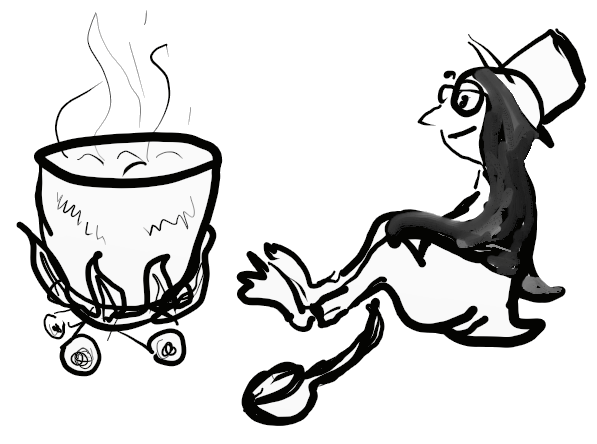
\epsfig{file=picts/gplt3/cook, width=.27\textwidth}
\end{wrapfigure}
В этом разделе собраны типичные примеры использования \gplt.
Для каждого примера приведены команда для запуска \gplt, сгенерированная им последовательность команд
для \gnuplot{} (получена с помощью опции \verb'-debug') и полученный в итоге рисунок.
Что бы не делать скриншоты экрана, все рисунки (если не сказано иное в случае генерации \pdf-файла) получены при помощи добавления
опций \verb'-sz .7 -to testXXX.png'. Опция \verb'-sz .7' нужна для уменьшения рисунка,
в \gnuplot{} размер задается в некоторых безразмерных <<попугаях>> относительно размера окна по умолчанию.
Для простых графиков размер по умолчанию слишком велик, при вставке двух рисунков рядом текст
в зарамочном оформлении получается слишком мелким. Размеры $0.6\div0.7$ позволяют вставлять два рисунка рядом в типичную полосу набора. 
Изображение в окне \gnuplot{} без \verb'-sz .7' будет отличаться только несколько большими размерами.



\section{Заключение}
\begin{wrapfigure}[7]{t}{.3\textwidth}
  \vphantom{.}
  \vspace{-2.3cm}

  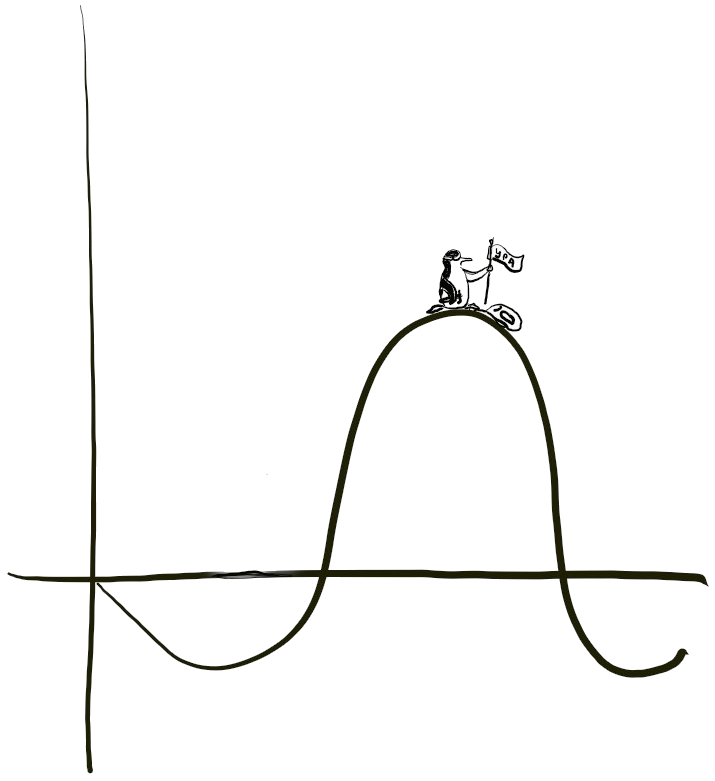
\epsfig{file=picts/gplt3/sin3, width=.27\textwidth}
\end{wrapfigure}

Трудно сказать, почему некоторые утилиты или языки программирования  получают всеобщее признание не смотря на все свои недостатки,
а другие, хотя будучи близкими к идеалу, остаются в забвении. 
Утилита \gplt{} конечно не идеальна, но она писалась <<для себя>>, под специфические запросы автора.
Подготовка рисунков для статей это всегда большая и кропотливая работа~---
абсолютное большинство рисунков для своих статей за последние 15 лет сделаны автором в \verb'gplt' различных версий.

Ключевым недостатком предыдущих версий \verb'gplt' являлось отсутсвие подробной документации,
\verb'gplt' использовали в основном некоторые из коллег, бывшие студенты автора, познакомившиеся с \verb'gplt'
в процессе обучения. Для \gplt{}  этот недостаток наконец исправлен. 

\bibliographystyle{myugost2008}
\bibliography{lit}

\end{document}
